
%(BEGIN_QUESTION)
% Copyright 2014, Tony R. Kuphaldt, released under the Creative Commons Attribution License (v 1.0)
% This means you may do almost anything with this work of mine, so long as you give me proper credit

In this phasor diagram, determine which phasor is {\it leading} and which is {\it lagging} the other:

$$\includegraphics[width=15.5cm]{i00840x01.eps}$$

\underbar{file i00840}
%(END_QUESTION)





%(BEGIN_ANSWER)

In this diagram, phasor ${\bf B}$ is leading phasor ${\bf A}$.  By convention, phasors normally rotate in the counter-clockwise direction.  If you envision the two arrow-tips of these phasors racing around in a circle like two race cars on a circular track, the one car that is ahead of the other is the one {\it leading} the race, while the one behind is the one {\it lagging}.

%(END_ANSWER)





%(BEGIN_NOTES)


%INDEX% Electronics review, phasor expressions of circuit quantities

%(END_NOTES)

